\documentclass[12pt,a4paper]{article}

\usepackage[a4paper,text={16.5cm,25.2cm},centering]{geometry}
\usepackage{lmodern}
\usepackage{amssymb,amsmath}
\usepackage{bm}
\usepackage{graphicx}
\usepackage{microtype}
\usepackage{hyperref}
\setlength{\parindent}{0pt}
\setlength{\parskip}{1.2ex}

\hypersetup
       {   pdfauthor = { Sheehan Olver },
           pdftitle={ foo },
           colorlinks=TRUE,
           linkcolor=black,
           citecolor=blue,
           urlcolor=blue
       }




\usepackage{upquote}
\usepackage{listings}
\usepackage{xcolor}
\lstset{
    basicstyle=\ttfamily\footnotesize,
    upquote=true,
    breaklines=true,
    breakindent=0pt,
    keepspaces=true,
    showspaces=false,
    columns=fullflexible,
    showtabs=false,
    showstringspaces=false,
    escapeinside={(*@}{@*)},
    extendedchars=true,
}
\newcommand{\HLJLt}[1]{#1}
\newcommand{\HLJLw}[1]{#1}
\newcommand{\HLJLe}[1]{#1}
\newcommand{\HLJLeB}[1]{#1}
\newcommand{\HLJLo}[1]{#1}
\newcommand{\HLJLk}[1]{\textcolor[RGB]{148,91,176}{\textbf{#1}}}
\newcommand{\HLJLkc}[1]{\textcolor[RGB]{59,151,46}{\textit{#1}}}
\newcommand{\HLJLkd}[1]{\textcolor[RGB]{214,102,97}{\textit{#1}}}
\newcommand{\HLJLkn}[1]{\textcolor[RGB]{148,91,176}{\textbf{#1}}}
\newcommand{\HLJLkp}[1]{\textcolor[RGB]{148,91,176}{\textbf{#1}}}
\newcommand{\HLJLkr}[1]{\textcolor[RGB]{148,91,176}{\textbf{#1}}}
\newcommand{\HLJLkt}[1]{\textcolor[RGB]{148,91,176}{\textbf{#1}}}
\newcommand{\HLJLn}[1]{#1}
\newcommand{\HLJLna}[1]{#1}
\newcommand{\HLJLnb}[1]{#1}
\newcommand{\HLJLnbp}[1]{#1}
\newcommand{\HLJLnc}[1]{#1}
\newcommand{\HLJLncB}[1]{#1}
\newcommand{\HLJLnd}[1]{\textcolor[RGB]{214,102,97}{#1}}
\newcommand{\HLJLne}[1]{#1}
\newcommand{\HLJLneB}[1]{#1}
\newcommand{\HLJLnf}[1]{\textcolor[RGB]{66,102,213}{#1}}
\newcommand{\HLJLnfm}[1]{\textcolor[RGB]{66,102,213}{#1}}
\newcommand{\HLJLnp}[1]{#1}
\newcommand{\HLJLnl}[1]{#1}
\newcommand{\HLJLnn}[1]{#1}
\newcommand{\HLJLno}[1]{#1}
\newcommand{\HLJLnt}[1]{#1}
\newcommand{\HLJLnv}[1]{#1}
\newcommand{\HLJLnvc}[1]{#1}
\newcommand{\HLJLnvg}[1]{#1}
\newcommand{\HLJLnvi}[1]{#1}
\newcommand{\HLJLnvm}[1]{#1}
\newcommand{\HLJLl}[1]{#1}
\newcommand{\HLJLld}[1]{\textcolor[RGB]{148,91,176}{\textit{#1}}}
\newcommand{\HLJLs}[1]{\textcolor[RGB]{201,61,57}{#1}}
\newcommand{\HLJLsa}[1]{\textcolor[RGB]{201,61,57}{#1}}
\newcommand{\HLJLsb}[1]{\textcolor[RGB]{201,61,57}{#1}}
\newcommand{\HLJLsc}[1]{\textcolor[RGB]{201,61,57}{#1}}
\newcommand{\HLJLsd}[1]{\textcolor[RGB]{201,61,57}{#1}}
\newcommand{\HLJLsdB}[1]{\textcolor[RGB]{201,61,57}{#1}}
\newcommand{\HLJLsdC}[1]{\textcolor[RGB]{201,61,57}{#1}}
\newcommand{\HLJLse}[1]{\textcolor[RGB]{59,151,46}{#1}}
\newcommand{\HLJLsh}[1]{\textcolor[RGB]{201,61,57}{#1}}
\newcommand{\HLJLsi}[1]{#1}
\newcommand{\HLJLso}[1]{\textcolor[RGB]{201,61,57}{#1}}
\newcommand{\HLJLsr}[1]{\textcolor[RGB]{201,61,57}{#1}}
\newcommand{\HLJLss}[1]{\textcolor[RGB]{201,61,57}{#1}}
\newcommand{\HLJLssB}[1]{\textcolor[RGB]{201,61,57}{#1}}
\newcommand{\HLJLnB}[1]{\textcolor[RGB]{59,151,46}{#1}}
\newcommand{\HLJLnbB}[1]{\textcolor[RGB]{59,151,46}{#1}}
\newcommand{\HLJLnfB}[1]{\textcolor[RGB]{59,151,46}{#1}}
\newcommand{\HLJLnh}[1]{\textcolor[RGB]{59,151,46}{#1}}
\newcommand{\HLJLni}[1]{\textcolor[RGB]{59,151,46}{#1}}
\newcommand{\HLJLnil}[1]{\textcolor[RGB]{59,151,46}{#1}}
\newcommand{\HLJLnoB}[1]{\textcolor[RGB]{59,151,46}{#1}}
\newcommand{\HLJLoB}[1]{\textcolor[RGB]{102,102,102}{\textbf{#1}}}
\newcommand{\HLJLow}[1]{\textcolor[RGB]{102,102,102}{\textbf{#1}}}
\newcommand{\HLJLp}[1]{#1}
\newcommand{\HLJLc}[1]{\textcolor[RGB]{153,153,119}{\textit{#1}}}
\newcommand{\HLJLch}[1]{\textcolor[RGB]{153,153,119}{\textit{#1}}}
\newcommand{\HLJLcm}[1]{\textcolor[RGB]{153,153,119}{\textit{#1}}}
\newcommand{\HLJLcp}[1]{\textcolor[RGB]{153,153,119}{\textit{#1}}}
\newcommand{\HLJLcpB}[1]{\textcolor[RGB]{153,153,119}{\textit{#1}}}
\newcommand{\HLJLcs}[1]{\textcolor[RGB]{153,153,119}{\textit{#1}}}
\newcommand{\HLJLcsB}[1]{\textcolor[RGB]{153,153,119}{\textit{#1}}}
\newcommand{\HLJLg}[1]{#1}
\newcommand{\HLJLgd}[1]{#1}
\newcommand{\HLJLge}[1]{#1}
\newcommand{\HLJLgeB}[1]{#1}
\newcommand{\HLJLgh}[1]{#1}
\newcommand{\HLJLgi}[1]{#1}
\newcommand{\HLJLgo}[1]{#1}
\newcommand{\HLJLgp}[1]{#1}
\newcommand{\HLJLgs}[1]{#1}
\newcommand{\HLJLgsB}[1]{#1}
\newcommand{\HLJLgt}[1]{#1}



\def\qqand{\qquad\hbox{and}\qquad}
\def\qqfor{\qquad\hbox{for}\qquad}
\def\D{ {\rm d} }
\def\I{ {\rm i} }
\def\E{ {\rm e} }
\def\C{ {\mathbb C} }
\def\R{ {\mathbb R} }
\def\CC{ {\cal C} }
\def\HH{ {\cal H} }
\def\vc#1{ {\mathbf #1} }
\def\bbC{ {\mathbb C} }

\def\qqqquad{\qquad\qquad}
\def\qqfor{\qquad\hbox{for}\qquad}
\def\qqwhere{\qquad\hbox{where}\qquad}
\def\Res_#1{\underset{#1}{\rm Res}\,}
\def\sech{ {\rm sech}\, }



\def\Xint#1{ \mathchoice
   {\XXint\displaystyle\textstyle{#1} }%
   {\XXint\textstyle\scriptstyle{#1} }%
   {\XXint\scriptstyle\scriptscriptstyle{#1} }%
   {\XXint\scriptscriptstyle\scriptscriptstyle{#1} }%
   \!\int}
\def\XXint#1#2#3{ {\setbox0=\hbox{$#1{#2#3}{\int}$}
     \vcenter{\hbox{$#2#3$}}\kern-.5\wd0} }
\def\ddashint{\Xint=}
\def\dashint{\Xint-}


\def\addtab#1={#1\;&=}
\def\ccr{\\\addtab}
\def\ip<#1>{\left\langle{#1}\right\rangle}
\def\dx{\D x}
\def\dt{\D t}
\def\dz{\D z}

\def\norm#1{\left\| #1 \right\|}

\def\abs#1{\left|{#1}\right|}
\def\fpr(#1){\!\pr({#1})}

\def\sopmatrix#1{ \begin{pmatrix}#1\end{pmatrix} }

\def\endash{–}
\def\mdblksquare{\blacksquare}

\begin{document}

\textbf{M3M6: Methods of Mathematical Physics}

Dr. Sheehan Olver

s.olver@imperial.ac.uk

\section{Lecture 3: Laurent series and residue calculus}
This lecture we cover

\begin{itemize}
\item[1. ] Fourier and Laurent series


\item[2. ] Contour integrals and Laurent coefficients


\item[3. ] Isolated singularities

\begin{itemize}
\item Residue at a point

\end{itemize}

\item[4. ] Contour integrals in domains with multiple holes

\begin{itemize}
\item The residue theorem

\end{itemize}

\item[5. ] Calculating integrals

\begin{itemize}
\item Application: Trigonometric integrals with rational functions

\end{itemize}
\end{itemize}
\subsection{Fourier and Laurent series}
\textbf{Definition (Fourier series)} On $[-\pi, \pi)$,  \emph{Fourier series} is an expansion of the form

\[
    g(\theta) = \sum_{k=-\infty}^\infty g_k \E^{i k \theta}
\]
where

\[
g_k = {1\over 2 \pi} \int_{-\pi}^\pi g(\theta) \E^{-i k \theta} d \theta
\]
\textbf{Definition (Laurent series)} In the complex plane, Laurent series around $z_0$ is an expansion of the form 

\[
    f(z) = \sum_{k=-\infty}^\infty f_k (z-z_0)^k 
\]
\textbf{Lemma (Fourier series = Laurent series)} On a circle in the complex plane 

\[
    C_r = \{z_0 + re^{i \theta} : -\pi \leq \theta < \pi \},
\]
Laurent series of $f(z)$ around $z_0$ converges for $z \in C_r$ if the Fourier series of $g(\theta) = f(z_0 + r e^{i \theta})$ converges, and the coefficients are given by

\[
f_k = {g_k \over r^k} = {1 \over 2 \pi i} \oint_{C_r} {f(\zeta) \over (\zeta - z_0)^{k+1}} d \zeta.
\]
\textbf{Proof}  This follows immediately from the change of variables $z = r \E^{\I \theta} + z_0$. \ensuremath{\blacksquare}

Interestingly, analytic properties of $f$ can be used to show decaying properties in $g$:

\subsection{Residue on a circle}
In this course, we will \emph{always} think of Laurent series living on a circle  $C_r(z_0) = \{z : |z-z_0| = r \}$.  That is,

\[
    f(z) \approx \sum_{k=-\infty}^\infty f_k (z-z_0)^k
\]
for $z \in C_r(z_0)$.  

\textbf{Proposition (Residue on a circle)}  Suppose the Laurent series is absolutely summable on $C_r(z_0)$. Then 

\[
\oint_{C_r(z_0)} f(z) dz = 2 \pi \I f_{-1}
\]
We refer to $f_{-1}$ as the residue over $C_r(z_0)$:

\[
\Res_{C_r(z_0)} f(z) := f_{-1} = {1 \over 2 \pi \I} \int_{C_r} f(z) \D z. 
\]
\emph{Example} For all $0 < r < \infty$, 

\[
\oint_{C_r} {1 \over z} dz = 2 \pi \I
\]
When $f$ is holomorphic in a neighbourhood of the circle, we can extend it to an annulus  (like Taylor series and disks):

\textbf{Proposition (Laurent series in an annulus)} Suppose $f$ is holomorphic in an open annulus $A_{\rho R}(z_0) = \{z : \rho  < | z - z_0| < R\}$.  Then the Laurent series converges uniformly in  any closed annulus inside $A_{\rho R}$

\emph{Proposition (Residue on a circle)} holds true regardless of the radius, that is, the  definition of $f_{-1}$ only depends on the annulus of analyticity:

\[
\Res_{A_{\rho R}(z_0)} f(z) := f_{-1} = {1 \over 2 \pi \I} \int_{C_r} f(z) \D z. 
\]
for any $\rho < r < R$. 

\subsection{Isolated singularities}
\textbf{Definition (isolated singularity)} $f$ has an  \emph{isolated singularity at} $z_0$ if it is holomorphic in an open annulus with inner radius 0: 

\[
A_{0R}(z_0) = \{z : 0 < |z - z_0| < R \}.
\]
\textbf{Definition (Removable singularity)} $f$ has a \emph{removable singularity at} $z_0$ if it has an isolated singularity at $z_0$ and all negative terms in the Laurent series in $A_{0R}(z_0)$ are zero:

\[
f(z) = f_0 + f_1 (z-z_0) + f_2 (z-z_0)^2 + \cdots
\]
Equivalently, $f$ has a removable singularity at $z_0$ if it is bounded as $z \rightarrow z_0$. 

An example would be a function like $f(z) = (\E^z - 1) / z$, which is analytic for $z \neq 0$ but is  not defined for $z = 0$. However, this singularity is artificial: we have from its Taylor series that 

\[
f(z) = (\E^{z} - 1)/z = (z + z^2 / 2! + \cdots)/z = 1 + z/2! + \cdots
\]
hence $f(z) \rightarrow 1$. We can therefore remove the singularity by taking $f_0$, the zeroth Laurent coefficent:

\[
\tilde f(z) = \begin{cases}
    (\E^z - 1)/ z & z \neq 0 \\
    1 & z = 0
    \end{cases}
\]
This construction is general:

\textbf{Proposition (Removing a removable singularity)} If  $f$ has a removable singularity at $z_0$ and $f_0$ is the zeroth Laurent coefficient

\[
    f_0 := {1 \over 2 \pi \I} \oint_{C_r(z_0)} {f(z) \over z} \D z
\]
for $r$ sufficiently small, then

\[
\tilde f(z) = \begin{cases} f_0 & z = z_0 \\
                                f(z) & 0 < |z-z_0| < R
                                \end{cases}
\]
is analytic in the disk $B_R(z_0) = \{ z : |z-z_0| < R \}$, with a convergent Taylor series. Hence the name.

\textbf{Definition (simple pole)} $f$ has a  \emph{simple pole at} $z_0$ if it is holomorphic in 

\[
  A_{0R}(z_0) = \{z : 0 < |z - z_0| < R \}
\]
with only one negative term in the Laurent series in $A_{0R}(z_0)$:

\[
  f(z) = {f_{-1} \over z - z_0}  + f_0 + f_1 (z - z_0) + \cdots
\]
where $f_{-1} \neq 0$.

\textbf{Definition (higher order pole)} $f$ has a  \emph{pole of order $N$ at} ${z_0}$ if it is holomorphic in 

\[
 A_{0R}(z_0) = \{z : 0 < |z - z_0| < R \}
\]
with only $N$ negative coefficients in the Laurent series:

\[
 f(z) = {f_{-N} \over (z - z_0)^N}  + {f_{1-N} \over (z - z_0)^{N-1}} +  \cdots + {f_{-1} \over z-z_0} + f_0 + f_1 (z-z_0) + \cdots
\]
where $f_{-N} \neq 0$.

\textbf{Definition (essential singularity)} $f$ has an \emph{essential singularity at} $z_0$ if it is holomorphic in $A_{0R}(z_0)$ and has an infinite number of negative Laurent coefficients.

An essential singularity is complicated but isolated, hence we can still calculate the integrals using Residue calculus.

\subsubsection{Residue at a point}
\textbf{Definition (Residue at a point)} Suppose $f$ has an isolated singularity at $z_0$, and is analytic in the annulus $A_{0R}(z_0)$ for some $R > 0$. Then we define the \emph{residue at} $z_0$ as

\[
{\underset{z = z_0}{\rm Res}}\, f(z) = {\underset{A_{0R}}{\rm Res}}\, f(z) = f_{-1}
\]
where $f_{-1}$ is the first negative coefficent of the Laurent series in $A_{0R}(z_0)$, that is, integrating over $C_r$ for any $0 < r < R$. 

\textbf{Proposition (Residue of ratio of analytic functions with simple pole)} Suppose

\[
f(z) = {A(z) \over B(z)}
\]
and $A$, $B$ are analytic/holomorphic in a disk of radius $R$ around $z_0$ and that $B$ has only a single zero at $z_0$:


\begin{align*}
A(z) = A_0 + A_1(z-z_0) + \cdots \cr
B(z) = B_1(z-z_0) + \cdots
\end{align*}
Then ${\underset{z = z_0}{\rm Res}}\, f(z) = {A_0 \over B_1}$

\textbf{Exercise (Residue of ratio of analytic functions with higher order  poles)} What is the residue at $z_0$ if $B$ has a higher order zero: $B(z) = B_N (z-z_0)^N + \cdots$?

\subsection{Contour integrals on domains with multiple holes}
Consider the following example:

\[
    {\sqrt{z-1}\sqrt{z+1} \over z^2 + 4}
\]
We still have the contour integral over a circle, and so \emph{Proposition (Residue on a circle)} still holds true for $r > 2$. But we can also deform the contour into three contours:


\begin{lstlisting}
(*@\HLJLk{using}@*) (*@\HLJLn{ApproxFun}@*)(*@\HLJLp{,}@*) (*@\HLJLn{Plots}@*)(*@\HLJLp{,}@*) (*@\HLJLn{ComplexPhasePortrait}@*)
(*@\HLJLn{f}@*) (*@\HLJLoB{=}@*) (*@\HLJLn{z}@*) (*@\HLJLoB{->}@*) (*@\HLJLnf{sqrt}@*)(*@\HLJLp{(}@*)(*@\HLJLn{z}@*)(*@\HLJLoB{-}@*)(*@\HLJLni{1}@*)(*@\HLJLp{)}@*)(*@\HLJLnf{sqrt}@*)(*@\HLJLp{(}@*)(*@\HLJLn{z}@*)(*@\HLJLoB{+}@*)(*@\HLJLni{1}@*)(*@\HLJLp{)}@*)(*@\HLJLoB{/}@*)(*@\HLJLp{(}@*)(*@\HLJLn{z}@*)(*@\HLJLoB{{\textasciicircum}}@*)(*@\HLJLni{2}@*)(*@\HLJLoB{+}@*)(*@\HLJLni{4}@*)(*@\HLJLp{)}@*)

(*@\HLJLn{\ensuremath{\Gamma}}@*) (*@\HLJLoB{=}@*) (*@\HLJLnf{Circle}@*)(*@\HLJLp{(}@*)(*@\HLJLnfB{1.1}@*)(*@\HLJLp{)}@*) (*@\HLJLoB{\ensuremath{\cup}}@*) (*@\HLJLnf{Circle}@*)(*@\HLJLp{(}@*)(*@\HLJLnfB{2.0}@*)(*@\HLJLn{im}@*)(*@\HLJLp{,}@*)(*@\HLJLnfB{0.1}@*)(*@\HLJLp{)}@*) (*@\HLJLoB{\ensuremath{\cup}}@*) (*@\HLJLnf{Circle}@*)(*@\HLJLp{(}@*)(*@\HLJLoB{-}@*)(*@\HLJLnfB{2.0}@*)(*@\HLJLn{im}@*)(*@\HLJLp{,}@*)(*@\HLJLnfB{0.1}@*)(*@\HLJLp{)}@*)
(*@\HLJLnf{phaseplot}@*)(*@\HLJLp{(}@*)(*@\HLJLoB{-}@*)(*@\HLJLnfB{2..2}@*)(*@\HLJLp{,}@*) (*@\HLJLoB{-}@*)(*@\HLJLnfB{3..3}@*)(*@\HLJLp{,}@*) (*@\HLJLn{f}@*)(*@\HLJLp{)}@*)
(*@\HLJLnf{plot!}@*)(*@\HLJLp{(}@*)(*@\HLJLn{\ensuremath{\Gamma}}@*)(*@\HLJLp{;}@*) (*@\HLJLn{color}@*)(*@\HLJLoB{=:}@*)(*@\HLJLn{black}@*)(*@\HLJLp{,}@*) (*@\HLJLn{label}@*)(*@\HLJLoB{=:}@*)(*@\HLJLn{contour}@*)(*@\HLJLp{,}@*) (*@\HLJLn{arrow}@*)(*@\HLJLoB{=}@*)(*@\HLJLkc{true}@*)(*@\HLJLp{,}@*) (*@\HLJLn{linewidth}@*)(*@\HLJLoB{=}@*)(*@\HLJLnfB{1.5}@*)(*@\HLJLp{)}@*)
\end{lstlisting}

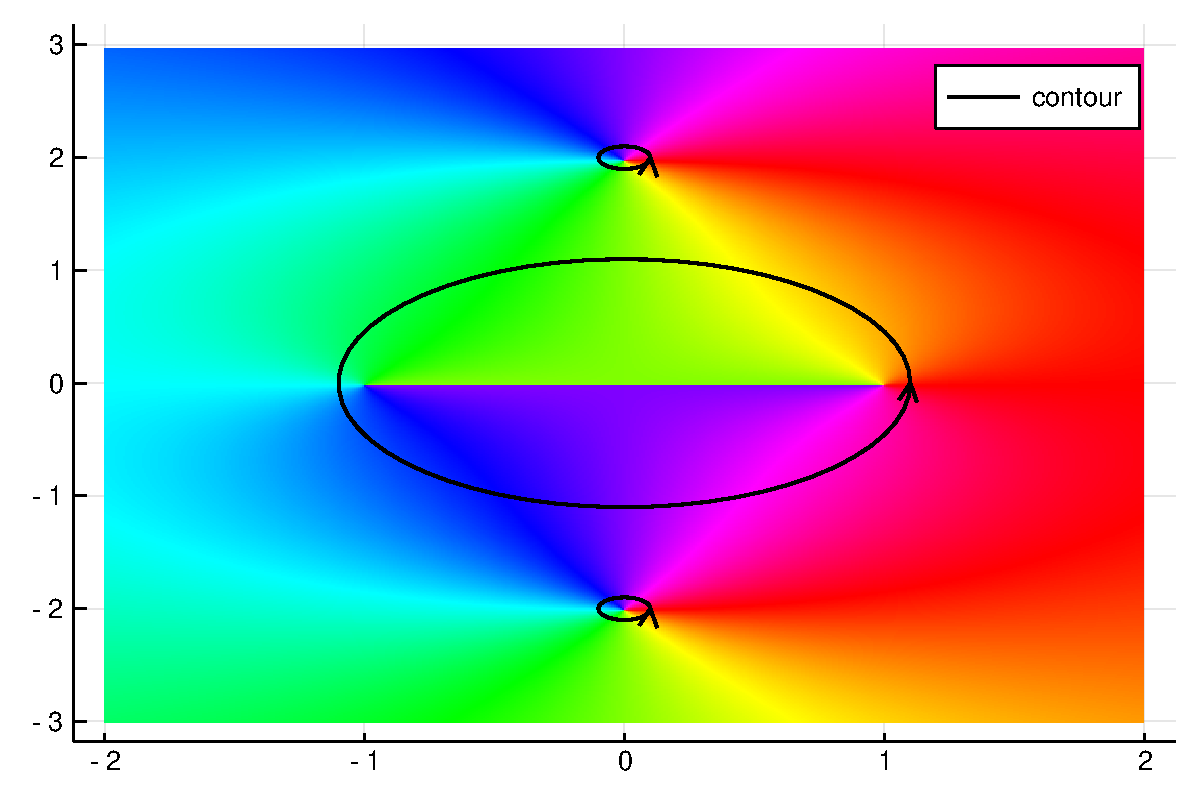
\includegraphics[width=\linewidth]{figures/Lecture3_1_1.pdf}

\begin{lstlisting}
(*@\HLJLnf{sum}@*)(*@\HLJLp{(}@*)(*@\HLJLnf{Fun}@*)(*@\HLJLp{(}@*)(*@\HLJLn{f}@*)(*@\HLJLp{,}@*) (*@\HLJLnf{Circle}@*)(*@\HLJLp{(}@*)(*@\HLJLnfB{2.1}@*)(*@\HLJLp{))),}@*) (*@\HLJLnf{sum}@*)(*@\HLJLp{(}@*)(*@\HLJLnf{Fun}@*)(*@\HLJLp{(}@*)(*@\HLJLn{f}@*)(*@\HLJLp{,}@*) (*@\HLJLn{\ensuremath{\Gamma}}@*)(*@\HLJLp{))}@*)
\end{lstlisting}

\begin{lstlisting}
(-8.270426731549189e-16 + 6.283185307179587im, -1.00975500904025e-15 + 6.28
3185307179586im)
\end{lstlisting}


Thus we can sum over three residues.

\subsubsection{Residue theorem}
\textbf{Theorem (Cauchy's Residue Theorem)} Let $f$ be holomprohic inside and on a simple closed, positively oriented contour $\gamma$ except at isolated points $z_1, \ldots, z_r$ inside $\gamma$. Then

\[
\oint_\gamma f(z) dz = 2 \pi i \sum_{j=1}^r {\underset{z = z_j}{\rm Res}}\, f(z)
\]
\subsection{Calculating integrals}
We can use the Residue theorem to calculate "hard" integrals. First, two trivial examples: consider

\[
f(z) = {\E^z \over z (z+2)}
\]
This has two simple poles, one at $z=0$ and one at $z = -2$, as seen clearly from the  phase portrait:


\begin{lstlisting}
(*@\HLJLn{f}@*) (*@\HLJLoB{=}@*) (*@\HLJLn{z}@*) (*@\HLJLoB{->}@*) (*@\HLJLnf{exp}@*)(*@\HLJLp{(}@*)(*@\HLJLn{z}@*)(*@\HLJLp{)}@*)(*@\HLJLoB{/}@*)(*@\HLJLp{(}@*)(*@\HLJLn{z}@*)(*@\HLJLoB{*}@*)(*@\HLJLp{(}@*)(*@\HLJLn{z}@*)(*@\HLJLoB{+}@*)(*@\HLJLni{2}@*)(*@\HLJLp{))}@*)
(*@\HLJLnf{phaseplot}@*)(*@\HLJLp{(}@*)(*@\HLJLoB{-}@*)(*@\HLJLnfB{3..3}@*)(*@\HLJLp{,}@*) (*@\HLJLoB{-}@*)(*@\HLJLnfB{3..3}@*)(*@\HLJLp{,}@*) (*@\HLJLn{f}@*)(*@\HLJLp{)}@*)
\end{lstlisting}

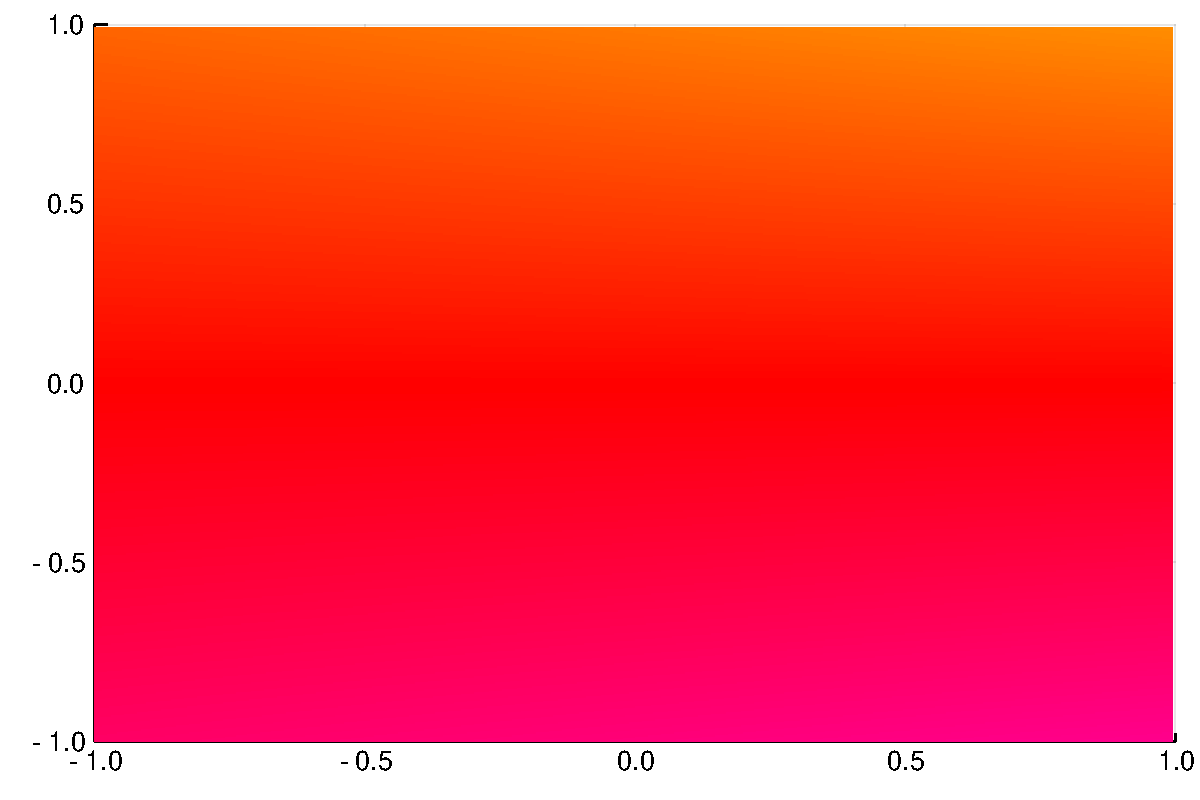
\includegraphics[width=\linewidth]{figures/Lecture3_3_1.pdf}

Consider integrating over $C_3$, a circle of radius 3 centred at the origin.  The residues are


\begin{align*}
\Res_{z=0} f(z) = \Res_{z=0}  {1 \over z} {\E^z \over z+2} = {1 \over 2} \\
\Res_{z=-2} f(z) = \Res_{z=-2}  {1 \over z+2} {\E^z \over z} = -{\E^{-2} \over 2}
\end{align*}
Thus the integral must be equal to $2 \pi \I (1/2 - \E^{-2} /2)$.  This matches a numerical approximation of the integral 


\begin{lstlisting}
(*@\HLJLnf{sum}@*)(*@\HLJLp{(}@*)(*@\HLJLnf{Fun}@*)(*@\HLJLp{(}@*)(*@\HLJLn{f}@*)(*@\HLJLp{,}@*) (*@\HLJLnf{Circle}@*)(*@\HLJLp{(}@*)(*@\HLJLnfB{3.0}@*)(*@\HLJLp{))),}@*) (*@\HLJLni{2}@*)(*@\HLJLn{\ensuremath{\pi}}@*)(*@\HLJLoB{*}@*)(*@\HLJLn{im}@*)(*@\HLJLoB{*}@*)(*@\HLJLp{(}@*)(*@\HLJLni{1}@*)(*@\HLJLoB{/}@*)(*@\HLJLni{2}@*) (*@\HLJLoB{-}@*) (*@\HLJLnf{exp}@*)(*@\HLJLp{(}@*)(*@\HLJLoB{-}@*)(*@\HLJLni{2}@*)(*@\HLJLp{)}@*)(*@\HLJLoB{/}@*)(*@\HLJLni{2}@*)(*@\HLJLp{)}@*)
\end{lstlisting}

\begin{lstlisting}
(-5.073166565789438e-16 + 2.716424322002157im, 0.0 + 2.716424322002157im)
\end{lstlisting}


A more complicated example is 

\[
f(z) = {\E^z \over z^2 (z+2)}
\]
which has a double pole at $z = 0$. We find the residue by expanding in Taylor series:

\[
 {1 \over z^2} {\E^z \over z +2} = {1 \over  2 z^2} (1 + z + O(z^2)) (1 - z/2 + O(z^2)) =
        {1 \over 2 z^2} + {1 \over 4 z} + O(1)
\]
That is,

\[
\Res_{z=0} f(z) = {1 \over 4} \qqand \Res_{z=-2} f(z) = {\E^{-2} \over 4}
\]
Again, residue calculus matches the numerical computation:


\begin{lstlisting}
(*@\HLJLnf{sum}@*)(*@\HLJLp{(}@*)(*@\HLJLnf{Fun}@*)(*@\HLJLp{(}@*)(*@\HLJLn{z}@*) (*@\HLJLoB{->}@*) (*@\HLJLnf{exp}@*)(*@\HLJLp{(}@*)(*@\HLJLn{z}@*)(*@\HLJLp{)}@*)(*@\HLJLoB{/}@*)(*@\HLJLp{(}@*)(*@\HLJLn{z}@*)(*@\HLJLoB{{\textasciicircum}}@*)(*@\HLJLni{2}@*)(*@\HLJLoB{*}@*)(*@\HLJLp{(}@*)(*@\HLJLn{z}@*)(*@\HLJLoB{+}@*)(*@\HLJLni{2}@*)(*@\HLJLp{)),}@*) (*@\HLJLnf{Circle}@*)(*@\HLJLp{(}@*)(*@\HLJLnfB{3.0}@*)(*@\HLJLp{))),}@*) (*@\HLJLni{2}@*)(*@\HLJLoB{*}@*)(*@\HLJLn{pi}@*)(*@\HLJLoB{*}@*)(*@\HLJLn{im}@*) (*@\HLJLoB{*}@*) (*@\HLJLp{(}@*)(*@\HLJLni{1}@*)(*@\HLJLoB{/}@*)(*@\HLJLni{4}@*) (*@\HLJLoB{+}@*) (*@\HLJLnf{exp}@*)(*@\HLJLp{(}@*)(*@\HLJLoB{-}@*)(*@\HLJLni{2}@*)(*@\HLJLp{)}@*)(*@\HLJLoB{/}@*)(*@\HLJLni{4}@*)(*@\HLJLp{)}@*)
\end{lstlisting}

\begin{lstlisting}
(-2.313334476762615e-16 + 1.7833804925887144im, 0.0 + 1.783380492588715im)
\end{lstlisting}



\end{document}
